
%!!! Calculations result and graphs here !!!%

\subsection{График зависимостей R(Q)}

Построил график для зависимостей R(Q) при разных температурах. \\График представлен на Рис. 3. \\

\begin{center}
    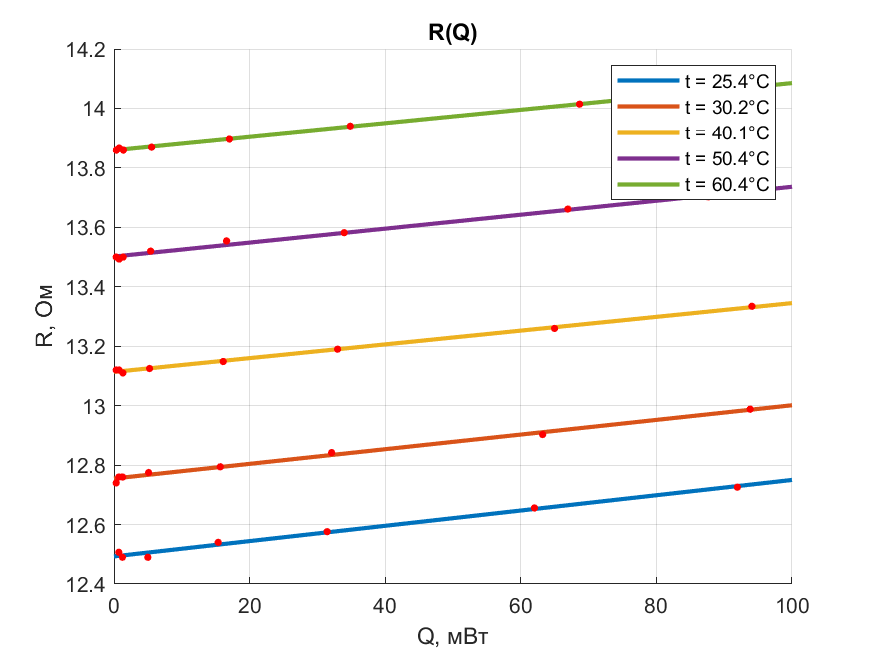
\includegraphics[scale = 1.3]{picks/223_R(Q).png} \\
    \textit{\textcolor[HTML]{000000}{Рис. 3. R(Q) для разных температур}}
\end{center}

\vspace{0.5cm}

    \begin{table}[h!]
    	\begin{center}
    		\caption*{\color[HTML]{000000}Таблица 2: Значения угловых к-тов \mth{\frac{dR}{dQ}} и значения R(0) для графика R(Q)}
    		\begin{tabular}{|P{3cm}|P{1.3cm}|P{1.3cm}|P{1.3cm}|P{1.3cm}|P{1.3cm}|}
    		\hline

                \mth{t, ^\circ C}    		& 25,4  & 30,2  & 40,1  & 50,4  & 60,4 \\  
    		    \hline
    		    R(0), Ом                    & 12,49 & 12,75 & 13,11 & 13,50 & 13,86 \\
    		    \hline
                \mth{\frac{dR}{dQ}, \frac{\text{Ом}}{\text{Вт}}}  & 2,57 & 2,46 & 2,31 & 2,34 & 2,25 \\


            \hline    		
    		\end{tabular}
    	\end{center}
    \end{table}

\newpage

\subsection{График зависимости R(t)}

Построил график для зависимости R(t). \\График представлен на Рис. 4. \\

\begin{center}
    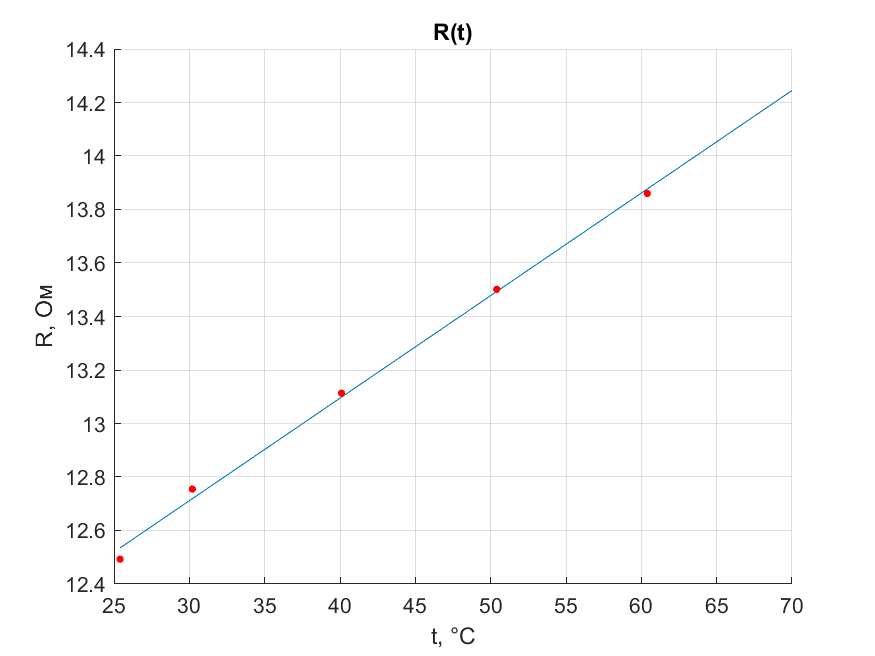
\includegraphics[scale = 1.3]{picks/223_R(T).png} \\
    \textit{\textcolor[HTML]{000000}{Рис. 4. R(t)}}
\end{center} 

\vspace{0.5cm}

Значение углового к-та для данного графика \mth{\frac{dR}{dT} = 3,83\cdot10^{-2} \frac{\text{Ом}}{K}}

\newpage

\subsection{Вычисление к-та теплопроводности при разных температурах термостата }

Из формулы (\ref{finalQ}) получил следующую формулу для расчета к: \\[0.2cm] 

\noindent\mth{k = \frac{\frac{dQ}{dR}\frac{dR}{dT}\,\cdot\, ln\frac{r_0}{r_1}}{2\pi L}} \\[0.2cm]

\noindent\mth{T_0} - Температура термостата; k - Значение теплопроводности. Результаты расчетов представлены в Таблице 3:

\begin{table}[h!]
    \begin{center}
        \caption*{\color[HTML]{000000}Таблица 3: к (T\mth{_0})}
        \begin{tabular}{|P{3cm}|P{1.3cm}|P{1.3cm}|P{1.3cm}|P{1.3cm}|P{1.3cm}|}
        \hline

            \mth{T_0, ^\circ C}    		         & 25,4  & 30,2  & 40,1  & 50,4  & 60,4 \\  
            \hline
            \mth{k, \frac{\text{Ом}}{\text{м}K} \cdot 10^{-2}} & 2,67 & 2,78 & 2,96 & 2,92 & 3,04 \\

        \hline    		
        \end{tabular}
    \end{center}
\end{table}

\subsection{График к(T)}

Пользуясь значениями из предыдущего пункта построил график к(T).\linebreak График представлен на рис. 5. \\

\begin{center}
    \includegraphics[scale = 1.0]{picks/223_k(T).png} \\
    \textit{\textcolor[HTML]{000000}{Рис. 5. k(t)}}
\end{center} 

\newpage

\subsection{Погрешности}

Привожу максимальные относительные погрешности для полученых величин: \\[0.2cm]

\noindent\mth{\epsilon_\frac{dR}{dQ} \approx 3,5 \%} - относительная погрешность для к-та наклона зависимости R(Q) \\

\noindent\mth{\epsilon_{R_0} \approx 0,1 \%} - относительная погрешность R(0) для зависимости R(Q) \\

\noindent\mth{\epsilon_\frac{dQ}{dT} \approx 3,8 \%} - относительная погрешность для производной полного потока тепла по температуре \\

\noindent\mth{\epsilon_k \approx 4,2 \%} - относительная погрешность для теплопроводности \\

\subsection{Подписаные данные}

Далее приложены фотографии данных на подписаных листах.
\newpage
\includepdf[pages={1, 2}]{data_proof1.pdf}